%%%%%%%%%%%%%%%%%%%%%%%%%%%%%%%%%%%%%%%%%
% baposter Landscape Poster
% LaTeX Template
% Version 1.0 (11/06/13)
%
% baposter Class Created by:
% Brian Amberg (baposter@brian-amberg.de)
%
% This template has been downloaded from:
% http://www.LaTeXTemplates.com
%
% License:
% CC BY-NC-SA 3.0 (http://creativecommons.org/licenses/by-nc-sa/3.0/)
%
%%%%%%%%%%%%%%%%%%%%%%%%%%%%%%%%%%%%%%%%%

%----------------------------------------------------------------------------------------
%	PACKAGES AND OTHER DOCUMENT CONFIGURATIONS
%----------------------------------------------------------------------------------------

\documentclass[a1paper,fontscale=0.5]{baposter} % Adjust the font scale/size here
\usepackage{mathtools}
\usepackage{graphicx} % support the \includegraphics command and options
\usepackage{caption}
\usepackage{subcaption}
\usepackage{wrapfig}
\usepackage[leftcaption]{sidecap}
\usepackage{lineno}
\usepackage{setspace}

\usepackage{graphicx} % Required for including images
%\graphicspath{{fig/}} % Directory in which figures are stored

\usepackage{amsmath} % For typesetting math
\usepackage{amssymb} % Adds new symbols to be used in math mode

\usepackage{booktabs} % Top and bottom rules for tables
\usepackage{enumitem} % Used to reduce itemize/enumerate spacing
\usepackage{palatino} % Use the Palatino font
\usepackage[font=small,labelfont=bf]{caption} % Required for specifying captions to tables and figures

\usepackage{multicol} % Required for multiple columns
\setlength{\columnsep}{1.5em} % Slightly increase the space between columns
\setlength{\columnseprule}{0mm} % No horizontal rule between columns

\usepackage{booktabs}

\usepackage{verbatim}
\usepackage[english]{babel}
\usepackage{times}
\usepackage{cinzel}
%\usepackage{arev}
\usepackage{lmodern}
\usepackage[T1]{fontenc}

\usepackage{tikz} % Required for flow chart
\usetikzlibrary{shapes,arrows} % Tikz libraries required for the flow chart in the template
\newcommand{\numberofreceptors}{ 28 }
\newcommand{\bonferroni}{ 11 }
\newcommand{\fdr}{ 26 }
\newcommand{\nocorrection}{ 2 }

\newcommand{\compresslist}{ % Define a command to reduce spacing within itemize/enumerate environments, this is used right after \begin{itemize} or \begin{enumerate}
\setlength{\itemsep}{1pt}
\setlength{\parskip}{0pt}
\setlength{\parsep}{0pt}
}

\definecolor{shadelightest}{rgb}{1, 0.86, 0.67} 
\definecolor{shadelighter}{rgb}{0.831, 0.655, 0.416} 

\definecolor{shade}{rgb}{0.667, 0.475, 0.224} 

\definecolor{shadedarker}{rgb}{0.502, 0.322, 0.082} 
\definecolor{shadedarkest}{rgb}{0.11, 0.095, 0.0} 


\usepackage{graphicx}
\begin{document}

\begin{poster}
{
headerborder=closed, % Adds a border around the header of content boxes
colspacing=1em, % Column spacing
bgColorOne=white, % Background color for the gradient on the left side of the poster
bgColorTwo=white, % Background color for the gradient on the right side of the poster
borderColor=shade, % Border color
headerColorOne=shadelightest, % Background color for the header in the content boxes (left side)
headerColorTwo=shadelightest, % Background color for the header in the content boxes (right side)
headerFontColor=shadedarkest, % Text color for the header text in the content boxes
boxColorOne=white, % Background color of the content boxes
textborder=rectangle, % Format of the border around content boxes, can be: none, bars, coils, triangles, rectangle, rounded, roundedsmall, roundedright or faded
eyecatcher=true, % Set to false for ignoring the left logo in the title and move the title left
headerheight=0.1\textheight, % Height of the header
headershape=rectangle, % Specify the rounded corner in the content box headers, can be: rectangle, small-rounded, roundedright, roundedleft or rounded
headerfont=\Large\bf\textsc, % Large, bold and sans serif font in the headers of content boxes
%textfont={\setlength{\parindent}{1.5em}}, % Uncomment for paragraph indentation
linewidth=2pt % Width of the border lines around content boxes
}
%----------------------------------------------------------------------------------------
%	TITLE SECTION 
%----------------------------------------------------------------------------------------
%
{
\includegraphics[height=5em]{fig/ICTP_logo}} % First university/lab logo on the left
{\huge \textsc{Odorant receptors are sensitive to molecular volume}} % Poster title
{\textsc{ Majid Saberi, Ali reza Vafaei Sadr, \bf{Hamed Seyed-allaei} \vspace{0.5em} }(hamed@ipm.ir)}
{
\includegraphics[height=5em]{fig/logo.jpg}} % First university/lab logo on the 
%\affiliation{G. Mill\'an Institute of Fluid Dynamics, Nanoscience and Industrial
%Mathematics, Universidad Carlos III de Madrid, Spain}


%----------------------------------------------------------------------------------------
%	Title
%----------------------------------------------------------------------------------------

\headerbox{}{name=ptitle,column=1, row=0}{

\cinzel
\begin{center}
\vspace{3cm}

{\Huge SCENT} 


--------\ {\small OF A}\ --------

{\Huge VOLUME}
\vspace{3cm}
\end{center}
}



%----------------------------------------------------------------------------------------
%	abstract
%----------------------------------------------------------------------------------------

\headerbox{Abstract}{name=abstract,column=0,row=0}{
%Which properties of a molecule define its odor? This is a basic question of olfaction, 
%yet to be answered. 
Human olfactory system has a repertoire of about 350 olfactory receptors. 
Molecules bind to them with different affinities and activate them with different efficacies, 
resulting in a combinatorial code that identifies odorants. 
We hypothesized that the binding affinity between a pair of odorant-receptor is affected by their relative sizes. 
The affinity can reaches its maximum if molecular volume of an odorant matches volume of a receptor's binding-pocket 
and it reach zero if the sizes are too different, 
obscuring the effect of other molecular properties. 
We formulated this hypothesis mathematically and verified it on experimental data.
%and predicted the volume and the structural flexibility of each receptor's binding-site, 
%which are significantly different among receptors. 
%This provides a reason for differences in smell among similar molecules of different sizes. 

\vspace{0.3em} % When there are two boxes, some whitespace may need to be added if the one on the right has more content
}

%----------------------------------------------------------------------------------------
%	REFERENCES
%----------------------------------------------------------------------------------------

\headerbox{References}{name=references,column=2,above=bottom}{
\small
\renewcommand{\section}[2]{\vskip 0.05em} % Get rid of the default "References" section title
%\nocite{} % Insert publications even if they are not cited in the poster
%\small{ % Reduce the font size in this block
%\bibliographystyle{unsrt}
%\bibliography{sample} % Use sample.bib as the bibliography file
 \begin{thebibliography}{1}

  \bibitem{saberi} Majid Saberi, Hamed Seyed-allaei, {
  Odorant receptors of Drosophila are sensitive to the molecular volume of odorants.}, 
  2016, Scientific Reports 6, DOI:10.1038/srep25103

  \bibitem{galizia} Galizia CG {\em et al.}, { Integrating heterogeneous odor response data into a common response model: A DoOR to the complete olfactome.}, 2010, Chemical Senses, DOI:10.1093/chemse/bjq042

 \bibitem{munch} Daniel Munch, C. Giovanni Galizia, {
DoOR 2.0 - Comprehensive Mapping of Drosophila melanogaster Odorant Responses.},
2016, Scientific Reports 6, DOI:10.1038/srep21841

 \bibitem{mainland}  Joel D Mainland {\em et al.}, {
Human olfactory receptor responses to odorants.},
2015, Scientific Data 2, DOI:10.1038/sdata.2015.2

 \bibitem{keller}  Keller {\em et al.}, {
 Predicting human olfactory perception from chemical features of odor molecules.},
2017, Science, DOI: 10.1126/science.aal2014. 


  \bibitem{Pedretti} Pedretti {\em et al.}, { VEGA - An open platform to develop chemo-bio-informatics applications, using plug-in architecture and script programming.}, 2004, Journal of Computer-Aided Molecular Design, DOI:10.1023/B:JCAM.0000035186.90683.f2

 \bibitem{zarzo} Manuel Zarzo, {\em Hedonic judgments of chemical compounds are correlated with molecular size.}, 2011, Sensors, DOI:10.3390/s110403667

  \end{thebibliography}
%}
}

%----------------------------------------------------------------------------------------
%	CONTACT INFORMATION
%----------------------------------------------------------------------------------------

%\headerbox{Contact Information}{name=contact,column=0,above=bottom}{ % This block is as tall as the references block

%\begin{description}\compresslist
%\item[Address] School of Cognitive Science,  Institute for Research in Fundamental Sciences (IPM),  Tehran, Iran
%\item[Email] hamed@ipm.ir
%\end{description}
%\begin{center}
%%\includegraphics[height=20mm]{fig/code.png}
%\end{center}
%}

%----------------------------------------------------------------------------------------
%	Introduction
%----------------------------------------------------------------------------------------

\headerbox{Assumptions}{name=assumptions,column=0, below=abstract}{ % This block's bottom aligns with the bottom of the conclusion block

%Survival of many species depends on their olfactory system. 
%They use it  to find food, 
%avoid poison, 
%escape from danger, 
%mate, 
%and bind to their offspring.
%An olfactory system detects volatile chemicals in the surrounding, 
%encodes the results and transmit them to limbic system and cortex.

%The front end of the olfactory system are olfactory receptor neurons.  
%Each neuron expresses only one kind of olfactory receptor (in insects they are co-expressed with Orco \cite{Larsson2004}).
%Neurons of the same type converge into the same glomeruli of the olfactory bulb (or antenatal lobe in insects),
%so that each glomerulus of olfactory bulb receives an amplified signal from only one type of olfactory receptor~\cite{root2007,Carey2011,Vosshall2000,Couto2005,fishilevich2005,gao2000,wang1998,mombaerts1996,vassar1994}.
%The olfactory systems use a combinatorial code: 
%unlike many other receptors which are activated by only specific ligands (eq. neurotransmitters and hormones),
%an olfactory receptor can be triggered by many odorant molecules, 
%and an odorant molecule can interact with different olfactory receptors~\cite{Malnic2000},

%The combinatorial code enables the olfactory system to discriminate trillion odors~\cite{Bushdid2014}.
%However, it is not clear yet which properties of a molecule contribute to its smell. It is a topic of ongoing researches and there are many theories~\cite{Turin,Keller2004,Araneda2000,Brookes2007,Franco2011,Pelz2006,Gabler2013,Schmuker2007,Haddad2008,Snitz2013,Yablonka2012,gane2013}.

%In this study, 
%we investigated the relation between molecular volumes of odorants and the responses of olfactory receptor neurons. 
%Our results suggest that molecular volume is a considerable factor, 
%but not the only factor that determines the neural response of the olfactory receptor neurons.

%The olfactory receptors are transmembrane proteins.
%In vertebrates, they are metabotropic receptors, they belong to the family of g-protein coupled receptor (GPCR). 
%Linda B. Buck and Richard Axel won the Nobel Prize in Physiology or Medicine, in 2004, 
%for its discovery ~\cite{Buck1991}.
%There are many similarities between the olfactory system of insects and vertebrates~\cite{Wilson2014,Kaupp2010}, 
%and it was assumed that insects use the same kind of signal transduction~\cite{Brody2000,Hill04102002}. 
%But recently, it has been argued that the olfactory receptors in insects are inotropic~\cite{Sato2008,Wicher2008,Nagel2011,Rong2011}, 	
%their topology is different from vertebrates~\cite{Benton2007,Smart2008},
%and they function in presence of another common receptor, called Orco~\cite{Larsson2004}.
%Regardless of the signal transduction, 
%all olfactory receptor have the same function, they have a binding-pocket (also known as binding-cavity and binding-site),
%where the ligands (odorants) bind to. 
%Binding to an odorant activates receptors and 
%the activated receptors changes the potential of the cell, 
%directly (inotropic) or indirectly (metabotropic).
%
%The amount of change in the membrane potential of an olfactory receptor neuron depends on the number of activated olfactory receptor proteins and the time that they remain activated,
%which are determined by various physio-chemical properties of the ligand (odorant) and the receptor~\cite{Turin,Araneda2000,Gabler2013,guerrieri2005,uchida2000}. 
%But here we focus on two properties: the volume and the flexibility of the binding-pocket.
%The molecular volume of a ligand should match the dimensions of the binding-pocket of the receptor,
%then it fits into the binding-pocket of the receptor and triggers the signal transduction. 
%Any mismatch in the volumes will affect the neural responses (Fig. \ref{fig:pocket-size}), 
%on the other hand the flexibility of the binding-pocket can compensate for the volume mismatch (Fig. \ref{fig:pocket-flex}).
%
%We could know the volume and flexibility of the binding-pocket, 
%if we knew its three dimensional structure.
%But this is not the case here, 
%as it is not easy to know the structure of integral proteins~\cite{Zhang2008,Lupieri2009}, 
%including olfactory receptors. 
%This is the topic of ongoing researches, 
%using various methods like Molecular Dynamic (MD) simulations, 
%mutagenesis studies, heterologus expression studies, and homology modeling~\cite{Khafizov2007,Man2004,Lai2005,Vaidehi2002,Floriano2004,Schmiedeberg2007,Katada2005,Kato2008,Rospars2013}.
%In this study, we use neural recording to predict the {\it in-vivo} volume and flexibility of binding-pocket of olfactory receptors.
%
%We suggest a functional relation between molecular volume and the neural responses, 
%we provide a methodology to estimate {\it molecular receptive range} or {\it tuning function} of olfactory receptors,
%and then we predict the structural properties of the binding-pocket of olfactory receptor - the volume and the flexibility of binding-pocket.
%Our results may help to select odorants  for new experimental studies, 
%may provide additional information about the structure of olfactory receptors to structural biologists, 
%and may contribute to the study of olfactory coding.
%
%To perform this study we use a public domain, 
%well structured database -- DoOR -- 
%that includes the neural responses of most olfactory receptors (OR) of Drosophila to many odorants~\cite{Galizia2010}. 
%This database aggregated data from many sources~\cite{Bruyne1999,Bruyne2001,Dobritsa2003,Goldman2005,Hallem2004,Hallem2006,
%Kreher2005,Kreher2008,Kwon2007,Pelz2006,Pelz2006,Schmuker2007,Stensmyr2003,
%Turner2009,VanderGoesvanNaters2007,Yao2005}.

When an odorant binds to a receptor, one of the following might happen:
\begin{center}
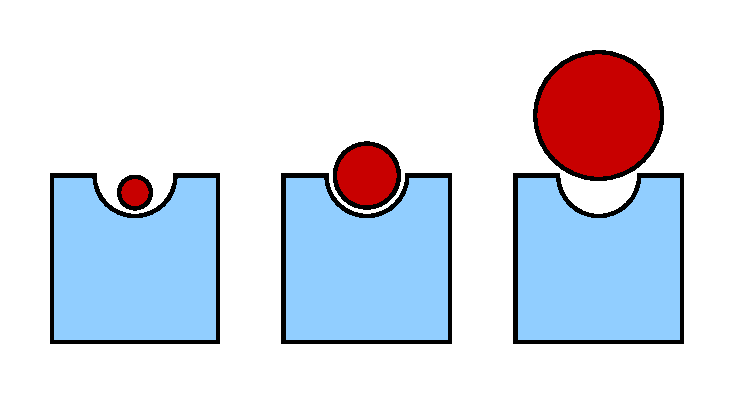
\includegraphics[width=0.65 \textwidth]{fig/binding-pocket-size} \\
\end{center}
Misfit because of small volume of molecule, perfect match and misfit because of large molecular volume.
\begin{center}
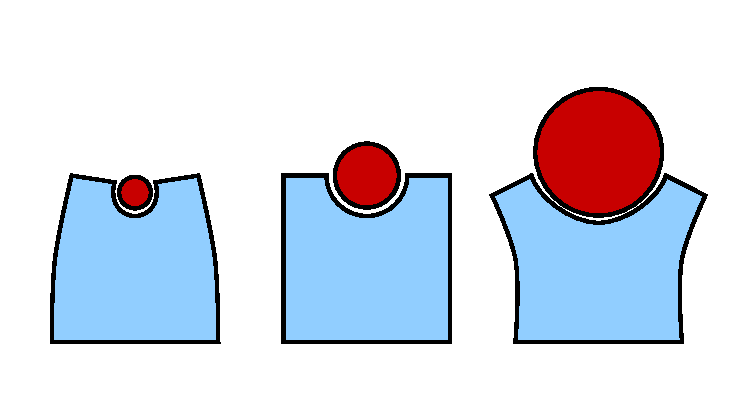
\includegraphics[width=0.65 \textwidth]{fig/binding-pocket-flex}
\end{center}
The flexibility of a receptor may compensate for the volume mismatches. 
The red disks are odorant molecule, 
and the blue shapes are olfactory receptor and binding-pocket.

Let assume the response $r_{nm}$ depends on the molecular volume of the odorant, $v_m$, and other physio-chemical properties of the molecule $m$; 
We assume that we can separate the response $r_{nm}$ into two terms:
%{\huge
\begin{equation}
	r_{nm} = f_n(v_m) \psi_{nm}. \nonumber
	\label{eqn:factors}
\end{equation}
%}
The first term, $f_n(v_m)$, depends only on the molecular volume of odorants.
The second term, $\psi_{nm}$ include every other influential properties of molecules, but the molecular volume.
Both terms are characteristic of each receptor, and they might vary from neuron to neuron.
}



%----------------------------------------------------------------------------------------
%	THE MATERIALS
%----------------------------------------------------------------------------------------

%\headerbox{Materials}{name=materials,column=0,below=assumptions}{
%
%\begin{center}
%%\includegraphics[width=0.1 \textwidth]{fig/DoOR-logo}
%\hfill
%%\includegraphics[height=0.1 \textwidth]{fig/VEGAZZ-logo}
%\hfill
%%\includegraphics[height=0.1 \textwidth]{fig/R_logo}
%\end{center}
%We take the neural data of DoOR database \cite{galizia} and we calculate molecular volume using a computational chemistry software -- VEGA ZZ~\cite{Pedretti}. 
%We used  GNU R to analyze the data.
%DoOR database can be summarized in an $N\times M$($55\times 251$) matrix. 
%Its elements, $r_{nm}$, are the response of neuron $n$ to odorant $m$. 
%This matrix is normalized between 0 and 1 so we have $0 \le r_{nm} \le 1$, where 1 is the strongest response.
%The only problem is that this matrix has many {\it Not Available} (NA) values, ~71\%,   
%and different neurons are excited by different set of odorants. 
%
%\begin{center}
%%\includegraphics[width=0.45 \textwidth]{fig/hist-volumes}
%\end{center}
%Density function of molecular volumes $g(v)$, considering all molecules of DoOR database. 
%The solid line is a Gaussian fit (Eq. \ref{eqn:hist-volumes}) and the dashed line shows the median, 
%which is slightly different from  the mean.
%
%}

%----------------------------------------------------------------------------------------
%	THE METHODS
%----------------------------------------------------------------------------------------

\headerbox{Experiment}{name=experiment,column=0, below=assumptions
%,row=0, bottomaligned=assumptions
}{
\includegraphics{fig/mainland.jpg}

Figure and data from Mainland et al \cite{mainland}
%Now we know the preferred volume $v_n$ of each receptor and also its flexibility $\sigma_n$.
}


%----------------------------------------------------------------------------------------
%	TESTS
%----------------------------------------------------------------------------------------

\headerbox{Histograms}{name=histograms,column=1,below=ptitle}{
\centering
\includegraphics[width = \textwidth]{fig/raw_histogram}
\includegraphics[width = \textwidth]{fig/cleaned_histogram}
\includegraphics[width = \textwidth]{fig/normalized_histogram}
}
\headerbox{Correlations}{name=correlations, column=1,below=histograms}{\centering
\begin{tabular}{|l|l|rr|rr|}
\toprule
    &      &       Luc &           &        RL &           \\ \hline
    &      &      0.0  &      10.0 &      0.0  &      10.0 \\
{} & Concentration &           &           &           &           \\
\midrule
Luc & 0.0  &  1.0 &  0.53 &  0.41 &  0.36 \\
    & 10.0 &  0.53 &  1.0 & -0.004 &  0.07 \\ \hline
RL & 0.0  &  0.41 & -0.004 &  1.0 &  0.88 \\
    & 10.0 &  0.36 &  0.07 &  0.88 &  1.0 \\
\bottomrule
\end{tabular}
}
\headerbox{Gaussian Naive Bayes}{name=GNB, column=1,below=correlations}{
\large
\begin{tabular}{|l|l|}
\hline 
features & accuracy \\ \hline
$ln(\frac{Luc}{RL})$ & 0.83  \\ 
$ln(Luc)$ & 0.91 \\
$ln(Luc)$ and $ln(RL)$ & 0.90 \\ \hline
\end{tabular}
}

\headerbox{Another Receptor}{name=Olfr73, column=1, below=GNB}{
\includegraphics[width= \textwidth]{fig/Olfr73}
}

%----------------------------------------------------------------------------------------
%	RESULTS AND DISCUSSIONS
%----------------------------------------------------------------------------------------

\headerbox{Results}{name=results,column=2
,row=0
}{

\begin{center}
%		\includegraphics[width= 1 \textwidth]{fig/vol-res-}
\end{center}
Response of olfactory receptors  versus molecular volume of odorants (circles), 
the fitted functions $f_n(v)$ from Eq.~\ref{eqn:factors} (solid lines), 
and the error bars of the mean of $f_n(v)$ (red vertical lines), 
for \numberofreceptors receptors that their response showed significant (p-value $<0.05$) dependence to molecular volume. 
Among them, \fdr are significant according to FDR correction (receptor names in bold) and 
\bonferroni are significant considering Bonferroni correction (receptor names in italic).
%\vspace{1em}

\begin{center}
		%\includegraphics[width=  0.49 \textwidth]{fig/mean-vol}
		%\includegraphics[width=  0.49 \textwidth]{fig/std-vol}
\end{center}
The preferred volumes of \numberofreceptors receptors $v_n$ (left). 
and their flexibilities $\sigma_n$ (right). 
The error bars are calculated using Jack-Knife method. 
%\vspace{1em}

\begin{center}
%\includegraphics[width= 0.825 \textwidth]{fig/pair-pval}
\end{center}
Pairs of olfactory receptors that differ significantly in their binding-pocket's volume (upper triangle) and flexibility (lower triangle).
			All blue shades have p-value of less than 0.05, 
			two darker shades have FDR corrected p-values of less than 0.05 and the darkest shade has Bonferroni corrected p-value of less than 0.05.
%\vspace{1em}

\begin{center}
%\includegraphics[width= 0.81 \textwidth]{fig/odorant-suggest}
\end{center}	
Venn diagram of DoOR database and our suggested important odorants of each receptor.
The database includes 240 molecules, 
some are used to study an olfactory receptor (blue areas), 
and data for the rests are not available (pink).
The hatched area are odorants with molecular volume close to the preferred volume of each receptor
($v_n \pm \frac{\sigma}{2}$).
We already know the neural response of hatched blue areas, 
but the hatched pink odorants could be the target of future experiments, we predict the rest give only zeros.


%There are two main assumption in this work: 
%First we assumed that the response of an olfactory receptor can be factorized into two terms, 
%according to (\ref{eqn:factors}).
%Second, we assumed that the volume dependence factor $f_n(v_m)$ in (\ref{eqn:factors}) 
%have a Gaussian form (Eq. \ref{eqn:volume-dependence}).
%Considering the physics and chemistry behind the binding-process (Fig. \ref{fig:binding-pocket}), 
%and the neural responses (Fig. \ref{fig:vol-res}), 
%these assumptions are logical. 

%but, to be sure, we also put them in a test. 
%After calculating function $f_n(v)$ for each olfactory receptor, we can calculate $\psi_{nm}$ of the equation \ref{eqn:factors}.
%If $\psi_{nm}$ is independent of molecular volumes, it means that the assumptions where justified.

%The function $f_n(v)$ can be considered as the tuning curve of olfactory receptor $n$ in response to molecular volume (Fig.~\ref{fig:vol-res}). 
%Each receptor has a preferred molecular volume $v_n$ and shows some flexibility $\sigma_n$. 
%The calculated $f_n(v)$ are in  Fig.~\ref{fig:vol-res}. 
%It includes \numberofreceptors receptors, 
%which show a significant dependence to molecular volume of odorants in their response (p-value $<0.05$).

%To address the multiple comparison problem, 
%we also calculated the level of significance according to both Bonferroni (very conservative) and FDR (less conservative) corrections. 
%From the results of \numberofreceptors receptors, 
%\bonferroni of them are significant according to Bonferroni correction (receptor names in italic), 
%\fdr of them are significant according to FDR correction 
%(receptor names in bold), 
%and the rest (\nocorrection receptors), 
%only satisfy the criteria of  p-value $<0.05$, without any corrections.
%Considering the FDR correction, 
%we can conclude that nearly half of receptors (\fdr / 60 ) show significant sensitivity toward molecular volumes. 
%The other half could be sensitive to molecular volume as well, but the current evidence are not enough and
%more experiments are necessary.

%The parameters of $f_n(v)$, $v_n$ and $\sigma_n$ are in Fig. \ref{fig:preferred_volume}.
%Figure \ref{fig:preferred_volume} demonstrate that the molecular volume preference of receptors are different (top). 
%and the flexibility of receptors are also different (bottom).
%To backup these claims, 
%we estimated the p-values of having different volume preference and flexibility for each pairs of \numberofreceptors receptors
%(Fig.~\ref{fig:p-values}). 
%From all possible 378 pairs, 
%when comparing the volume preferences, 
%133 have a p-value of less than 0.05, 
%this number reduces to 89 after using FDR and further reduces to 32 using Bonferroni correction.
%When comparing flexibilities, 
%the numbers become 168, 134 and 77 respectively. 
%The union of these two set says that 226 (p-value $<0.05$), 171 (FDR corrected), and 91 (Bonferroni corrected) pairs of receptors showed distinct differences in their binding-pocket characteristics.
%
%This diversity is important in perceiving the quality of smells. 
%In a hypothetical experiment, 
%assume that every characteristic of odorant molecules are the same but their molecular volume.
%If all olfactory receptors had the same preferred volume and flexibility, 
%any change in the molecular volume would change only the intensity of smell not its quality.
%But olfactory receptors have different preferred volumes and flexibilities, 
%so any change in the molecular volume of an odorant results in a different combinatorial encoding which affects the quality of perceived smell as well its intensity.
%This agrees with the work of M. Zarzo: larger molecules  smell better~\cite{zarzo2011}.
%That may describe the difference in the smell of methanol, ethanol, propanol and butanol. 
%Methanol smells pungent, ethanol smells pleasant and winy, propanol and butanol smell like ethanol except butanol  has a little banana like aroma.
%The molecular volume affects the combinatorial encoding, 
%and the combinatorial code determines the quality of odorants.
%
%Here we showed that the responses of olfactory receptor neurons are related to the molecular volume of odorants, 
%apart from that, it is not clear which other features of molecules are measured by olfactory receptors. 
%There are many works that try to connect the physio-chemical properties of molecules to the evoked neural response or perceived smells.
%But the non-linear volume dependence (Eq. \ref{eqn:factors} and Eq. \ref{eqn:volume-dependence})  
%may mask important relations between molecules and neural responses.
%When $f_n(v)$ is zero or close to zero, 
%the value of $\psi_{nm}$ does not matter. 
%
%We predict odorants with a molecular volume on the tails of $f_n(v)$ goes undetected, 
%regardless of any other physio-chemical properties that they may have. 
%This prediction can be confirmed in furthur experiments. 
%
%To better study $\psi_{nm}$ of a receptor, 
%it is better to have many data points and those data points are better to be around the preferred volume of the receptor.
%But this is not the case in current data. 
%For many receptors, 
%most data points are on the tails of $f_n(v)$, which is close to zero.
%We have suggested the best selection of odorants for each of \numberofreceptors studied receptors 
%(see Venn diagram in Fig.~\ref{fig:odorant-suggest} and supplemental file proposed-odorants.csv), 
%saving time and expenses of future experiments. 

%After gathering enough data, 
%by considering the effect of molecular volume on the response of olfactory receptor neurons, 
%one might discover more subtle dependence between other molecular features and neural responses, 
%by investigating $\psi_{nm}$, 
%which otherwise would be masked by this non-linear relation $f_n(v)$.

%We also predict some {\it in-vivo} structural aspects of  the binding-pocket of olfactory receptors:
%the preferred volume of each receptor results from the volume of the binding-pocket,
%the flexibility of a receptor results from the rigidity or flexibility of the binding-pocket; 
%%Therefore, our results provides information about both structural and dynamical properties of olfactory receptors in Drosophila. 
%These data add some constrains over the 3d structure of olfactory receptors, 
%which may help the prediction and calculation of 3d structure of these proteins. 

%The method of this work can be combined with mutagenesis as well. 
%Some genes of an olfactory receptor are mutated, 
%then its response to a selection of molecules are measured and finally the preferred volume and flexibility are calculated.
%In this way we can understand which amino acids of the olfactory receptor contribute to the volume and flexibility of the binding-pocket, 
%as well as affecting the function of the receptors.
%
%There is one possible improvment to this work. Approximating $f_n(v)$ and $g(v)$ with a Gaussian function makes the mathematical formulation simple and readable. 
%But a semi-infinite function may be a better choice for molecular volumes which can not have negative values.
%
%Although this work is on the data of Drosophila, 
%we expect that the general principles and methodologies of this work hold for vertebrates as well. 
%But considering the similarities and dissimilarities between insects and vertebrate, 
%this should be verified.

}


\end{poster}

\end{document}
